\documentclass[conference,a4paper]{APSIPA2026}
\usepackage{amsmath}
\usepackage{graphicx}
\usepackage{multirow}
\usepackage{threeparttable}
\usepackage[backend=biber,style=ieee,]{biblatex}
\addbibresource{mybib.bib}

%\setlength{\voffset}{-2.0cm}
%\setlength{\hoffset}{-1cm}

\usepackage{geometry}
\geometry{a4paper, top=19mm, bottom=43mm, right=13mm, left=13mm}
% \geometry{a4paper, top=19.1mm, bottom=43.1mm, right=13mm, left=13mm, columnsep=0.241in}
% Optional setting if the PDF file couldn't pass the IEEE Xplore format examination.

\usepackage{fancyhdr}
\renewcommand{\headrulewidth}{0pt}
\renewcommand{\footrulewidth}{0pt}
\fancypagestyle{firststyle}{
  \fancyhf{}
  \fancyhead[C]{2026 Asia Pacific Signal and Information Processing Association Annual Summit and Conference (APSIPA ASC)}
}

\begin{document}

\title{Guidelines for APSIPA ASC 2026 Manuscripts}

\author{
\authorblockN{
Author 1\authorrefmark{1} and
Author 2\authorrefmark{2}
}

\authorblockA{
\authorrefmark{1}
Vietnam National University, Hanoi, Vietnam \\
E-mail: xx@vnu.edu.vn  Tel/Fax: +84-XXXXXXXX}

\authorblockA{
\authorrefmark{2}
Hanoi University of Science and Technology, Vietnam \\
E-mail: yy@hust.edu.vn  Tel/Fax: +84-XXXXXXXX}
}

\maketitle
\thispagestyle{firststyle}
\pagestyle{empty}

\begin{abstract}
  This document is an example of what your manuscript to APSIPA ASC 2026 should look like.
  Authors are asked to conform to the directions reported in this document.
\end{abstract}

\begin{IEEEkeywords}
  Signal, information processing, aligning human-machine generalization. 
\end{IEEEkeywords} 

\section{Introduction}
This document shows guidelines for preparing a manuscript in the proceedings of APSIPA ASC 2026.
The format here described allows for a graceful transition to the style required for that publication.

\section{General Instructions}
Prepare your paper in full-size format on A4 paper (210mm by 297mm).
% Prepare your paper in full-size format on US Letter paper (8 1/2 by 11 inches).
Write the paper in English.

We kindly ask authors to check your paper if all fonts in the PDF file of the manuscript are embedded and subset.
It can be checked from Document Properties/Fonts in File menu of Adobe Acrobat.

\subsection{Paper Length}
The length of the paper is limited to {\bf 4 to 6 pages} (including everything).
{\bf Please DO NOT put a page number on each page}.

\subsection{Type Sizes and Typefaces}
Follow the type sizes specified in Table I.
As an aid in gauging type size, 1 point is about 0.35 mm.
The size of the lowercase letter ``j'' will give the point size.
Times New Roman is the preferred font.

\begin{table}[b]
\begin{center}
\begin{threeparttable}
\caption{Type size for papers}
\begin{tabular}{|c|p{40mm}|c|c|}
\hline
\multirow{3}{6mm}{\centering Type size (pts.)}
& \multicolumn{3}{c|}{\rule[-5pt]{0pt}{14pt} Appearance}\\
\cline{2-4}
& \multicolumn{1}{c|}{\rule[-5pt]{0pt}{16pt}Regular} & Bold & Italic\\
\hline
6 & Table captions,\tnote{a}\quad table subscripts & & \\
\cline{2-4}
8 & Section titles,\tnote{a}\quad references, tables, table
names,\tnote{a}\quad first letters in table
captions,\tnote{a}\quad figure captions, footnotes, text
subscripts, and superscripts
& & \\
\cline{2-4}
9 & & Abstract & \\
\cline{2-4}
10 & Authors,  affiliations, main text,
equations, first letters in section titles\tnote{a}\quad
& & Subheading \\
\cline{2-4}
11 & Authors' names & & \\
\cline{2-4}
24 & Paper title   & & \\
\hline
\end{tabular}
\begin{tablenotes}
\item[a] Uppercase
\end{tablenotes}
\end{threeparttable}
\end{center}
\end{table}

\subsection{Margins}
top = 19mm, bottom = 43mm and left = right = 13mm.
The column width is 8mm (3.45 in).
The space between the two columns is 4mm (0.17 in).
Paragraph indentation is 3.5 mm (0.14 in).

% top = 0.75 inches, bottom = 1 inch and left = right = 0.625 inches.
% The column width is 3.5 inches.
% The space between the two columns is 0.25 inches.
% Paragraph indentation is 3.5 mm (0.14 in).

\subsection{Style}
The style of the paper is single-spaced two-column format like this sample.
Left- and right-justify your columns.
Use tables and figures to adjust column length.
On the last page of your paper, adjust the lengths of the columns so that they are equal.
Use automatic hyphenation and check spelling.
Digitize or paste down figures.

\subsection{The First Page}
Center the title across both columns at the top of the first page, followed by authors' names and their affiliations.
Long title should be typed on two lines without a blank line intervening.

The two-column format should start with the abstract.
Type the abstract at the beginning of the left column in the first page, leaving approximately 1 cm (0.39 in) from the title part.
The abstract should be the same as that submitted electronically on the symposium website.

Begin typing the main body of the text immediately after the abstract, observing the two-column format as shown in this example.

\section{Helpful Hints}
\subsection{Figures and Tables}

Position figures and tables at the tops and bottoms of columns near where they are first discussed.
Avoid placing them in the middle of columns or at the end of the paper.
Large figures and tables may span across both columns.

Figure captions should be centered below the figures; table captions should be centered above.
Avoid placing figures and tables before their first mention in the text.
Use the abbreviation ``Fig. 1,'' even at the beginning of a sentence.

\begin{figure}[t]
\begin{center}
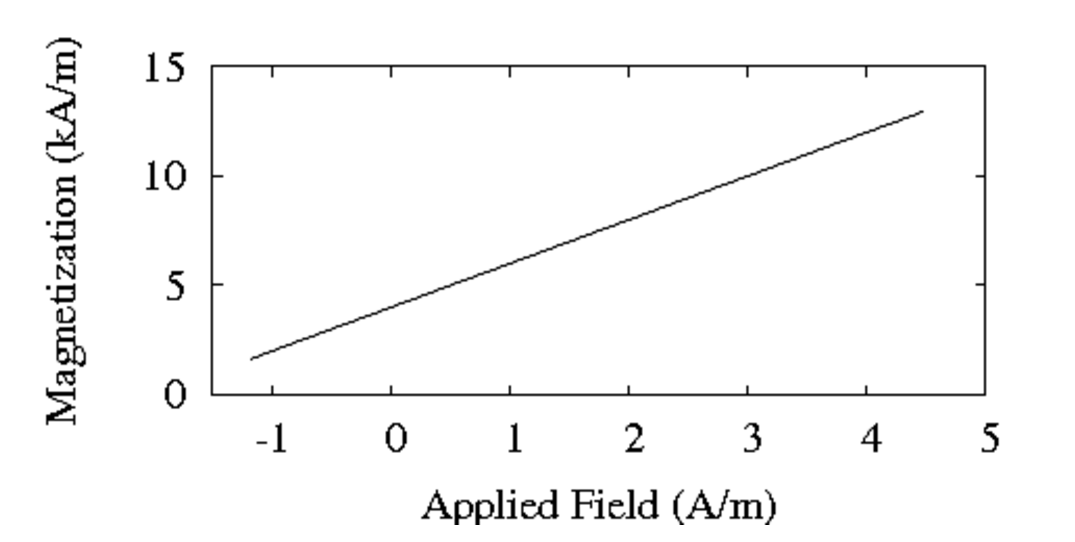
\includegraphics[width=70mm]{Fig1-Times-Roman.eps}
%\includegraphics[width=70mm]{Fig1-TimesNewRomanPSMT.eps}
%\fbox{ \rule[-17mm]{0pt}{30mm} FIGURE }
\end{center}
\caption{Magnetization as a function of applied field.}
\vspace*{-3pt}
{\hfill\footnotesize Note how the caption is centered in the column.\hfill}
\end{figure}

Figure axis labels are often a source of confusion.
Use words rather than symbols.
For example, write ``Magnetization,'' or ``Magnetization (M)'' not just ``M.''  Put units in parentheses.
Do not label axes only with units.
In the example, write ``Magnetization (A/m)'' or ``Magnetization (A $\cdot$ m$^{-1}$).''
Do not label axes with a ratio of quantities and units.
For example, write ``Temperature (K),'' not ``Temperature/K.''

Multipliers can be especially confusing.
Write ``Magnetization (kA/m)'' or ``Magnetization ($10^3$ A/m).''
Figure labels should be legible, about 10-point type.

\subsection{References}
Number citations consecutively in square brackets \cite{eason1955certain}.
Punctuation follows the bracket \cite{maxwell1873treatise}.
Refer simply to the reference number, as in \cite{jacobs1963fine}.
Use ``Ref. \cite{jacobs1963fine}'' or ``Reference \cite{jacobs1963fine}'' at the beginning of a sentence: ``Reference \cite{jacobs1963fine} was the first ...''

Gather the full set of references together in the section of references.
Place the section of references before any appendices, unless they contain references.
Arrange the references in alphabetical order or in order of appearance in the paper.

Give all authors' names; use ``et al.''  if there are six authors or more.
Papers that have not been published, even if they have been submitted for publication, should be cited as ``unpublished'' \cite{title_of_paper_if_known}.
Papers that have been accepted for publication should be cited as ``in press'' \cite{title_of_paper_with_only_first_word_capitalized}.
In a paper title, capitalize the first word and all other words except for conjunctions, prepositions less than seven letters, and prepositional phrases.

For papers published in translated journals, first give the English citation, then the original foreign-language citation \cite{4549593}.

\subsection{Appendices}
Although conference papers do not normally have an appendix, appendices, if any, directly follow the text and the references, (but see IV.B).
Letter them in sequence and provide an informative title: {\bf Appendix A Title of Appendix}.

\subsection{Footnote}
Number footnotes separately in superscripts like this\footnote{This is how a footnote should appear.}.
Place the actual footnote at the bottom of the column in which it was cited.
Footnotes should be separated from the text by a line\footnote{Note the line separating the footnotes from the text.}.
Do not put footnotes in the reference list.
Use letters for table footnotes (see Table I).

\subsection{Abbreviations and Acronyms}
Define abbreviations and acronyms the first time they are used in the text, even if they have been defined in the abstract.
Abbreviations such as APSIPA, SI, MKS, CGS, ac, dc, and rms do not have to be defined.
Do not use abbreviations in the title unless they are unavoidable.

\subsection{Equations}
Number equations consecutively with equation numbers in parentheses flush with the right margin, as in (1).
To make your equations more compact, you may use the solidus ( / ), the exp function, or appropriate exponents.
Italicize Roman symbols for quantities and variables, but not Greek symbols.
Use an en dash ( $-$ ) rather than a hyphen for a minus sign.
Use parentheses to avoid ambiguities in denominators.
Punctuate equations with commas or periods when they are part of a sentence, as in

\begin{equation}
 a + b = c.
\end{equation}

Symbols in your equation should be defined before the equation appears or immediately following.
Use ``(1),'' not ``Eq. (1)'' or ``equation (1),'' except at the beginning of a sentence: ``Equation (1) is ...''

\subsection{Other Recommendations}
The Roman numerals used to number the section headings are optional.
If you do use them, do not number {\scshape{Acknowledgment}} and {\scshape{References}}, and begin Subheadings with letters.

Use two spaces after periods (full stops).
Hyphenate complex modifiers: ``zero-field-cooled magnetization.''
Avoid dangling participles, such as, ``Using (1), the potential was calculated.''
Write instead, ``The potential was calculated using (1),'' or ``Using (1), we calculated the potential.''


% \renewcommand{\textheight}{98mm}


Use a zero before decimal points: ``0.25,'' not ``.25.''
Use ``cm$^3$,'' not ``cc.''
Do not mix complete spellings and abbreviations of units: ``Wb/m$^2$'' or ``webers per square meter,'' not ``webers/m$^2$.''
Spell units when they appear in text: ``...a few henries,'' not ``...a few H.''
If your native language is not English, try to get a native English-speaking colleague to proofread your paper.
Do not add page numbers.

%\newpage
\section{Units}

Use either SI (MKS) or CGS as primary units. (SI units are encouraged.)
English units may be used as secondary units (in parentheses).
An exception would be the use of English units as identifiers in trade, such as ``3.5-inch disk drive.''

Avoid combining SI and CGS units, such as current in amperes and magnetic field in oersteds.
This often leads to confusion because equations do not balance dimensionally.
If you must use mixed units, clearly state the units for each quantity that you use in an equation.

\section{Some Common Mistakes}
The word ``data'' is plural, not singular.
The subscript for the permeability of vacuum$_0$ is zero, not a lowercase letter ``o.''
In American English, periods and commas are within quotation marks, ``like this period.''
A parenthetical statement at the end of a sentence is punctuated outside of the closing parenthesis (like this).
(A parenthetical \emph{sentence} is punctuated within the parentheses.)
A graph within a graph is an ``inset,'' not an ``insert.''
The word alternatively is preferred to the word ``alternately'' (unless you mean something that alternates).
Do not use the word ``essentially'' to mean ``approximately'' or ``effectively.''
Be aware of the different meanings of the homophones ``affect'' and ``effect,'' ``complement'' and ``compliment,'' ``discreet'' and ``discrete,'' ``principal'' and ``principle.''
Do not confuse ``imply'' and ``infer.''
The prefix ``non'' is not a word; it should be joined to the word it modifies, usually without a hyphen.
There is no period after the ``et'' in the Latin abbreviation ``et al.''
The abbreviation ``i.e.''  means ``that is,'' and the abbreviation ``e.g.''  means ``for example.''
An excellent style manual for science writers is \cite{young2002technical}.


\section{Conclusions}
The conclusion goes here.

\section*{Acknowledgment}
The preferred spelling of the word ``acknowledgment'' in America is without an ``e'' after the ``g.''
Try to avoid the stilted expression, ``One of us (R. B. G.) thanks ...''
Instead, try ``R.B.G. thanks ...''
Put sponsor acknowledgments in the unnumbered footnote on the first page.

% \begin{thebibliography}{1}

% \bibitem{1}
% G.~Eason, B.~Noble, and I.~N.~Sneddon, ``On certain integrals of
% Lipschitz-Hankel type involving products of Bessel functions,''
% \emph{Phil. Trans. Roy. Soc. London,} vol. A247, pp. 529-551, April
% 1955.

% \bibitem{2}
% J.~Clerk~Maxwell, \emph{A Treatise on Electricity and Magnetism,}
% 3$^{\rm rd}$ ed., vol. 2. Oxford: Clarendon, 1892, pp.68-73.

% \bibitem{3}
% I.~S.~Jacobs and C.~P.~Bean, ``Fine particles, thin films and exchange
% anisotropy,'' in \emph{Magnetism,} vol. III, G.T. Rado and H. Suhl,
% Eds. New York: Academic, 1963, pp. 271-350.

% \bibitem{4}
% K.~Elissa, ``Title of paper if known,'' unpublished.

% \bibitem{5}
% R.~Nicole, ``Title of paper with only first word capitalized,''
% \emph{J. Name Stand. Abbrev.,} in press.

% \bibitem{6}
% Y.~Yorozu, M.~Hirano, K.~Oka, and Y.~Tagawa, ``Electron spectroscopy
% studies on magneto-optical media and plastic substrate interface,''
% \emph{APSIPA Transl. J. Magn. Japan,} vol. 2, pp. 740-741, August 1987
% [\emph{Digests 9$^{\rm th}$ Annual Conf. Magnetics Japan,} p. 301,
% 1982].

% \bibitem{7}
% M.~Young, \emph{The Technical Writer's Handbook.} Mill Valley, CA:
% University Science, 1989.

% \end{thebibliography}

\printbibliography

\end{document}
